\documentclass[12pt,a4paper]{article}

% ---- Pakete ----
\usepackage[T1]{fontenc}
\usepackage[utf8]{inputenc}
\usepackage[ngerman]{babel}
\usepackage{amsmath, amssymb}
\usepackage{graphicx}
\usepackage{booktabs}
\usepackage{hyperref}
\usepackage[margin=2.5cm]{geometry}
\usepackage{parskip}
\usepackage[backend=bibtex, style=numeric-comp, sorting=none]{biblatex}
\addbibresource{refs.bib}

% ---- Kopf/Fuß ----
\usepackage{fancyhdr}
\pagestyle{fancy}
\fancyhf{}
\fancyhead[L]{F-Praktikum — Supraleitung}
\fancyhead[R]{Marks, Sporrer}
\fancyfoot[C]{\thepage}

% ---- Metadaten ----
\hypersetup{
    pdftitle={F-Praktikum: Supraleitung},
    pdfauthor={Sebastian Marks, Simon Sporrer},
    colorlinks=true, linkcolor=blue, citecolor=blue, urlcolor=blue,
}

% ====================================================================
\begin{document}

% ---- Titelseite ----
\begin{titlepage}
    \centering
    \vspace*{2cm}
    {\LARGE\bfseries F-Praktikum\\[0.4em]
    \Huge Supraleitung\par}
    \vspace{1.5cm}
    {\large Versuchsdurchführung: Sommersemester 2026\par}
    \vspace{3cm}
    {\large
    \textbf{Sebastian Marks}\\[0.3em]
    \textbf{Simon Sporrer}\\[1.5em]
    Fakultät für Physik\\
    Universität Regensburg\par}
    \vfill
    {\large\today\par}
\end{titlepage}

% ---- Inhaltsverzeichnis ----
\tableofcontents
\newpage

% ---- Kapitel ----
% ============================================================
%  Kapitel 1 — Einleitung
% ============================================================
\section{Einleitung}

Supraleitung ist eines der faszinierendsten Phänomene der Festkörperphysik: Unterhalb einer materialspezifischen kritischen Temperatur $T_c$ verschwindet der elektrische Widerstand eines Leiters vollständig, und das Material expelliert das Magnetfeld aus seinem Inneren
(Meißner-Ochsenfeld-Effekt)~\cite{Meissner1933}.
Seit der Entdeckung der Supraleitung in Quecksilber durch Heike Kamerlingh Onnes im Jahr 1911 hat das Phänomen die Grundlagenforschung sowie zahlreiche technologische Anwendungen~--- von Kernspin\-tomographen über Teilchenbeschleuniger bis zu supraleitenden Quantencomputern~--- maßgeblich geprägt.

Das mikroskopische Verständnis gelang erst 1957 durch Bardeen, Cooper und Schrieffer
(BCS-Theorie~\cite{BCS1957}): Elektronen bilden unterhalb von $T_c$ über phononvermittelte Wechselwirkung Cooperpaare mit Gesamtimpuls null; diese kondensieren in einen kollektiven Grundzustand, der elektrischen Widerstand verhindert.
Eine phänomenologische Beschreibung des Magnetfeldverhaltens liefern die London-Gleichungen~\cite{London1935}, die unter anderem den Meißner-Effekt quantitativ erklären.
Eine Erweiterung auf temperaturabhängige Ordnungsparameter bietet die Ginzburg-Landau-Theorie, die den Übergang in supraleitende Dünne-Film-Geometrien besonders zugänglich macht.

Mit der Entdeckung der Hochtemperatur-Supraleitung in Kuprat-Verbindungen durch Bednorz und Müller~\cite{Bednorz1986} erweiterte sich das Anwendungsgebiet erheblich: Die Sprungtemperaturen liegen weit über dem Siedepunkt von Stickstoff ($77~\mathrm{K}$), was kostengünstige Kryotechnik ermöglicht.

Im vorliegenden F-Praktikumversuch werden grundlegende Eigenschaften der klassischen Typ-I-Supraleitung an einem dünnen Bleifilm ($\mathrm{Pb}$, $100~\mathrm{nm}$) bei Temperaturen nahe dem Siedepunkt von flüssigem Helium ($T \approx 4{,}2~\mathrm{K}$) untersucht.
Konkret werden das magnetische Phasendiagramm $B_c(T)$, das die Grenze zwischen supraleitendem und normalem Zustand beschreibt, sowie der kritische Strom $I_c(T)$ als Funktion der Temperatur gemessen.
Beide Größen folgen innerhalb der Ginzburg-Landau-Theorie charakteristischen Potenzgesetzen, die an die Messdaten angepasst werden.
Ergänzend wird das Levitationsphänomen an einem YBCO-Hochtemperatursupraleiter qualitativ beobachtet.

\medskip\noindent
\textbf{Gliederung.}
Kapitel~\ref{sec:theorie} legt die theoretischen Grundlagen der Typ-I- und Typ-II-Supraleitung dar.
Der Versuchsaufbau wird in Kapitel~\ref{sec:aufbau} beschrieben.
Die Auswertung der $B_c(T)$- und $I_c(T)$-Messungen erfolgt in Kapitel~\ref{sec:auswertung}, gefolgt von Diskussion und Fazit in Kapitel~\ref{sec:diskussion}.

\newpage

% ============================================================
%  Kapitel 2 — Theorie
% ============================================================
\section{Theoretische Grundlagen}
\label{sec:theorie}

\subsection{Phänomenologische Eigenschaften}

Supraleiter zeichnen sich durch zwei charakteristische Eigenschaften aus:
(i) \emph{Verschwindender Widerstand}: Unterhalb von $T_c$ ist der Gleichstromwiderstand exakt null.
(ii) \emph{Meißner-Ochsenfeld-Effekt}: Ein Magnetfeld, das zuvor in das Material eingedrungen war, wird beim Übergang in den supraleitenden Zustand vollständig aus dem Inneren des Leiters verdrängt~\cite{Meissner1933}.
Dieser Effekt zeigt, dass Supraleitung kein bloß widerstandsloser Zustand ist, sondern ein echter thermodynamischer Zustand mit perfektem Diamagnetismus.

\subsection{London-Gleichungen}

Fritz und Heinz London~\cite{London1935} beschrieben das elektromagnetische Verhalten von Supraleitern durch zwei Gleichungen.
Die zweite London-Gleichung verknüpft den Superstrom $\mathbf{J}_s$ mit dem Magnetfeld $\mathbf{B}$:
\begin{equation}
    \nabla \times \mathbf{J}_s = -\frac{1}{\mu_0 \lambda_L^2}\,\mathbf{B},
    \label{eq:london2}
\end{equation}
wobei die London'sche Eindringtiefe
\begin{equation}
    \lambda_L = \sqrt{\frac{m_e}{\mu_0\, n_s\, e^2}}
    \label{eq:lambda}
\end{equation}
die charakteristische Längenskala angibt, auf der ein äußeres Magnetfeld exponentiell in den Supraleiter abfällt.
$n_s$ ist die Dichte der Cooperpaare.
Für Blei gilt bei $T \to 0$: $\lambda_L^{\,\mathrm{Pb}}(0) \approx 39~\mathrm{nm}$.

\subsection{Typ-I-Supraleitung und das kritische Feld $B_c(T)$}

Beim Typ-I-Supraleiter (z.\,B.\ Blei) gibt es genau ein kritisches Magnetfeld $B_c(T)$.
Für $B < B_c$ befindet sich das Material im Meißner-Zustand (vollständige Feldverdrängung), für $B > B_c$ ist die Supraleitung zerstört.
Die Temperaturabhängigkeit folgt empirisch und im Rahmen der Ginzburg-Landau-Theorie dem parabolischen Gesetz
\begin{equation}
    B_c(T) = B_c(0)\left[1 - \left(\frac{T}{T_c}\right)^2\right].
    \label{eq:bc_parabola}
\end{equation}
Für Blei sind die Bulk-Werte: $B_c(0) \approx 80~\mathrm{mT}$ und $T_c \approx 7{,}2~\mathrm{K}$~\cite{Buckel2013}.

\subsubsection*{Dünne Filme im senkrechten Magnetfeld}

Für einen dünnen supraleitenden Film der Dicke $d$ (mit $d \ll \lambda_L$) in einem senkrecht zur Filmoberfläche angelegten Magnetfeld erhöht sich das effektive kritische Feld gegenüber dem Bulk erheblich.
Die effektive Eindringtiefe des dünnen Films, auch Pearl-Länge genannt~\cite{Pearl1964}, ist
\begin{equation}
    \Lambda = \frac{2\lambda_L^2}{d},
\end{equation}
was für $d < 2\lambda_L$ zu $\Lambda > \lambda_L$ führt.
Das geometrisch bedingte Demagnetisierungsfeld bewirkt, dass ein weit höheres äußeres Feld angelegt werden muss, um die Supraleitung zu unterdrücken.
Experimentell werden bei dünnen Pb-Filmen in senkrechter Geometrie kritische Felder im Bereich von $\sim 0{,}1~\mathrm{T}$ bis mehreren Tesla beobachtet~\cite{Tinkham2004}.

\subsection{Kritischer Strom $I_c(T)$}

Neben dem kritischen Feld gibt es einen kritischen Strom $I_c(T)$.
Übersteigt die Stromdichte den kritischen Wert $J_c$, wird durch den selbsterzeugten Magnetfluss die Supraleitung lokal zerstört.
Im Rahmen der Ginzburg-Landau-Theorie gilt in der Nähe von $T_c$:
\begin{equation}
    I_c(T) \propto \left(1 - \frac{T}{T_c}\right)^n,
    \label{eq:ic_gl}
\end{equation}
wobei der Exponent $n$ von der genauen Geometrie und dem Regime abhängt (typisch $n \approx 1{,}5$ bis $2$).

\subsection{Typ-II-Supraleitung und YBCO}

Typ-II-Supraleiter besitzen zwei kritische Felder $B_{c1}$ und $B_{c2}$.
Für $B < B_{c1}$ besteht der Meißner-Zustand; für $B_{c1} < B < B_{c2}$ dringt das Feld in Form quantisierter Flussschläuche (Vortices) ein (Shubnikov-Phase), ohne die Supraleitung global zu zerstören.
Erst für $B > B_{c2}$ ist die Supraleitung vollständig unterdrückt.

Yttrium-Barium-Kuprat (YBa$_2$Cu$_3$O$_{7-\delta}$, YBCO) ist ein Hochtemperatur-Typ-II-Supraleiter mit $T_c \approx 92~\mathrm{K}$ und extrem hohen kritischen Feldern ($B_{c2} > 100~\mathrm{T}$).
Die supraleitenden Eigenschaften sind stark anisotrop: In der $ab$-Ebene der CuO$_2$-Schichten ist die Leitfähigkeit deutlich größer als entlang der $c$-Achse~\cite{Buckel2013}.

\subsection{Flux-Pinning und Levitation}

Durch Flux-Pinning~--- das Festhalten von Vortices an Defekten im Material~--- kann ein Typ-II-Supraleiter ein eingedrungenes Magnetfeld auch nach Abkühlung unterhalb von $T_c$ fixieren (Field-Cooling).
Dieses Phänomen ermöglicht stabile Levitation: Ein Magnet kann sowohl über als auch unter einem YBCO-Supraleiter schwebend gehalten werden, ohne zu fallen oder anzuhaften.

\newpage

% ============================================================
%  Kapitel 3 — Versuchsaufbau und Durchführung
% ============================================================
\section{Versuchsaufbau und Durchführung}
\label{sec:aufbau}

\subsection{Kryostat und Temperaturregelung}

Alle Messungen am Bleifilm wurden in einem Helium-Kryostaten bei Temperaturen von $T \approx 5{,}8~\mathrm{K}$ bis $T \approx 7{,}2~\mathrm{K}$ durchgeführt.
Der Kryostat ist mit flüssigem Helium gefüllt ($T_\mathrm{Siede} = 4{,}2~\mathrm{K}$) und thermisch durch ein Helium-Gas-Polster gegen die Außenwelt isoliert.
Die Temperatur der Probe wird durch einen elektrischen Heizdraht im Probenraum eingestellt und von einem Cernox-Widerstandsthermometer (Lakeshore~340 Temperatur\-regler, Eingang~B) auf $\pm 5~\mathrm{mK}$ genau gemessen und geregelt.

\subsection{Bleifilm-Probe}

Die Probe besteht aus einem $100~\mathrm{nm}$ dicken Bleifilm, der auf einem Substrat durch Aufdampfen hergestellt wurde.
Die elektrischen Kontakte sind als Vierpunkt-Anordnung ausgeführt: Zwei äußere Kontakte injizieren den Messstrom, zwei innere Kontakte messen die Spannung über den supraleitenden Bereich des Films.
Durch diese Methode wird der Einfluss von Kontakt- und Zuleitungswiderständen eliminiert.

\subsection{Messaufbau $B_c(T)$}

Das Magnetfeld wird von einem supraleitenden Magneten (Cryomagnetics~4G, GPIB-Adresse~2) erzeugt, der senkrecht zur Filmfläche orientiert ist.
Die Feldrampe erfolgt mit einer Rate von $\dot{I} = 0{,}05~\mathrm{A/s}$, entsprechend $\dot{B} = 0{,}05~\mathrm{A/s} \times 0{,}10524~\mathrm{T/A} = 5{,}262~\mathrm{mT/s}$.

Der Messstrom durch den Film wird von einem Yokogawa~GS200-Spannungsquellengerät mit einem Vorwiderstand von $R_\mathrm{pre} = 100~\mathrm{k}\Omega$ erzeugt; bei $U_\mathrm{Yoko} = 10~\mathrm{V}$ ergibt sich ein Strom von
\begin{equation}
    I_\mathrm{mess} = \frac{10~\mathrm{V}}{100~\mathrm{k}\Omega} = 100~\mu\mathrm{A}.
\end{equation}
Die Spannung am Film wird von einem HP~3458A-Multimeter mit einem Spannungsverstärker ($\times 10$) aufgenommen.
Die Datenerfassung erfolgt mit dem Messprogramm \textit{Lab::Moose} (Perl), das alle Messwerte im Sekundentakt aufzeichnet.

\paragraph{Hinweis zur B-Feld-Rekonstruktion.}
Im Mess-Skript war die direkte Auslesung des Ist-Magnetfeldes ($\mathtt{get\_imag}$) aus Kompatibilitätsgründen auskommentiert.
Die B-Feld-Spalte in den Messdateien enthält daher stets den Wert $B = 0$.
Das tatsächliche Feld wird aus der Messzeit rekonstruiert:
\begin{equation}
    B(t) = \dot{B} \cdot t = 5{,}262~\frac{\mathrm{mT}}{\mathrm{s}} \cdot t.
    \label{eq:b_recon}
\end{equation}
Die Konsistenz dieser Rekonstruktion wurde anhand der beobachteten Übergangslängen und der Sweepzeit überprüft.

\subsection{Messaufbau $I_c(T)$}

Für die $I_c(T)$-Messungen wird das Yokogawa~GS200 als Spannungsquelle mit einem kleineren Vorwiderstand $R_\mathrm{pre} = 1~\mathrm{k}\Omega$ betrieben, sodass Ströme bis $I_\mathrm{max} = 4~\mathrm{mA}$ erreichbar sind.
Bei jeder Temperatur wird $I$ von $0$ bis $I_\mathrm{max}$ in Schritten von $\Delta I = 20~\mu\mathrm{A}$ gerampt; die Filmspannung $U$ wird mit dem HP~3458A aufgezeichnet.
Der kritische Strom $I_c$ wird als derjenige Wert bestimmt, bei dem $U$ um mehr als $500~\mu\mathrm{V}$ über die SC-Basislinie ($U_0 \approx 290~\mu\mathrm{V}$, aus Kontaktwiderstand und Thermospannung) ansteigt.

\subsection{Nicht durchgeführte Versuche}

Die Messung der magnetischen Suszeptibilität mittels induktiver Pickup-Spule (Versuchsteil~A.2) konnte nicht durchgeführt werden, da der entsprechende Versuchsaufbau zum Versuchstermin nicht funktionsfähig war.
Ebenso wurden die Widerstands-Temperatur-Kurven von YBCO in $ab$- und $c$-Richtung (Versuchsteil~B) nicht gemessen, da kein entsprechender Stickstoff-Kryostat zur Verfügung stand.
Das Levitationsexperiment (Versuchsteil~C) wurde qualitativ beobachtet, jedoch ohne quantitative Auswertung oder fotografische Dokumentation.

\newpage

% ============================================================
%  Kapitel 4 — Auswertung
% ============================================================
\section{Auswertung}
\label{sec:auswertung}

\subsection{Magnetisches Phasendiagramm $B_c(T)$ des Bleifilms}

\subsubsection*{Spannungstransitionen $U(B)$}

Abbildung~\ref{fig:vb_curves} zeigt die gemessenen Spannungskurven $U(B)$ des Bleifilms bei 16 verschiedenen Temperaturen zwischen $T = 5{,}82~\mathrm{K}$ und $T = 7{,}20~\mathrm{K}$.
Das Magnetfeld wurde dabei gemäß Gleichung~\eqref{eq:b_recon} aus der Messzeit rekonstruiert.

Im supraleitenden Zustand beträgt die gemessene Spannung $U_\mathrm{SC} \approx 290~\mu\mathrm{V}$, was einem Restwiderstands-Offset aus Zuleitungs- und Kontaktwiderständen entspricht.
Im normalleitenden Zustand liegt die Spannung bei $U_N \approx 7{,}1~\mathrm{mV}$, entsprechend einem Filmwiderstand von $R_N = U_N / I_\mathrm{mess} = 7{,}1~\mathrm{mV} / 100~\mu\mathrm{A} \approx 71~\Omega$.

Für Temperaturen $T \geq 6{,}796~\mathrm{K}$ ist der Film bereits bei $B = 0$ normalleitend; die Filmtemperatur liegt damit über der Null-Feld-Sprungtemperatur des Films.
Bei $T = 5{,}821~\mathrm{K}$ bleibt der Film innerhalb des gesamten Messbereichs ($B_\mathrm{max} \approx 505~\mathrm{mT}$) supraleitend; das kritische Feld liegt damit oberhalb dieser Grenze.

Das kritische Feld $B_c$ wird bei jeder Temperatur als diejenige Feldstärke bestimmt, bei der die Spannung die 50\%-Schwelle
\begin{equation}
    U_{50\%} = \tfrac{1}{2}(U_\mathrm{SC} + U_N)
    \label{eq:uc50}
\end{equation}
überschreitet.
Durch lineare Interpolation zwischen den angrenzenden Datenpunkten ergibt sich eine Genauigkeit von $\Delta B_c \lesssim 5~\mathrm{mT}$.

\begin{figure}[htbp]
    \centering
    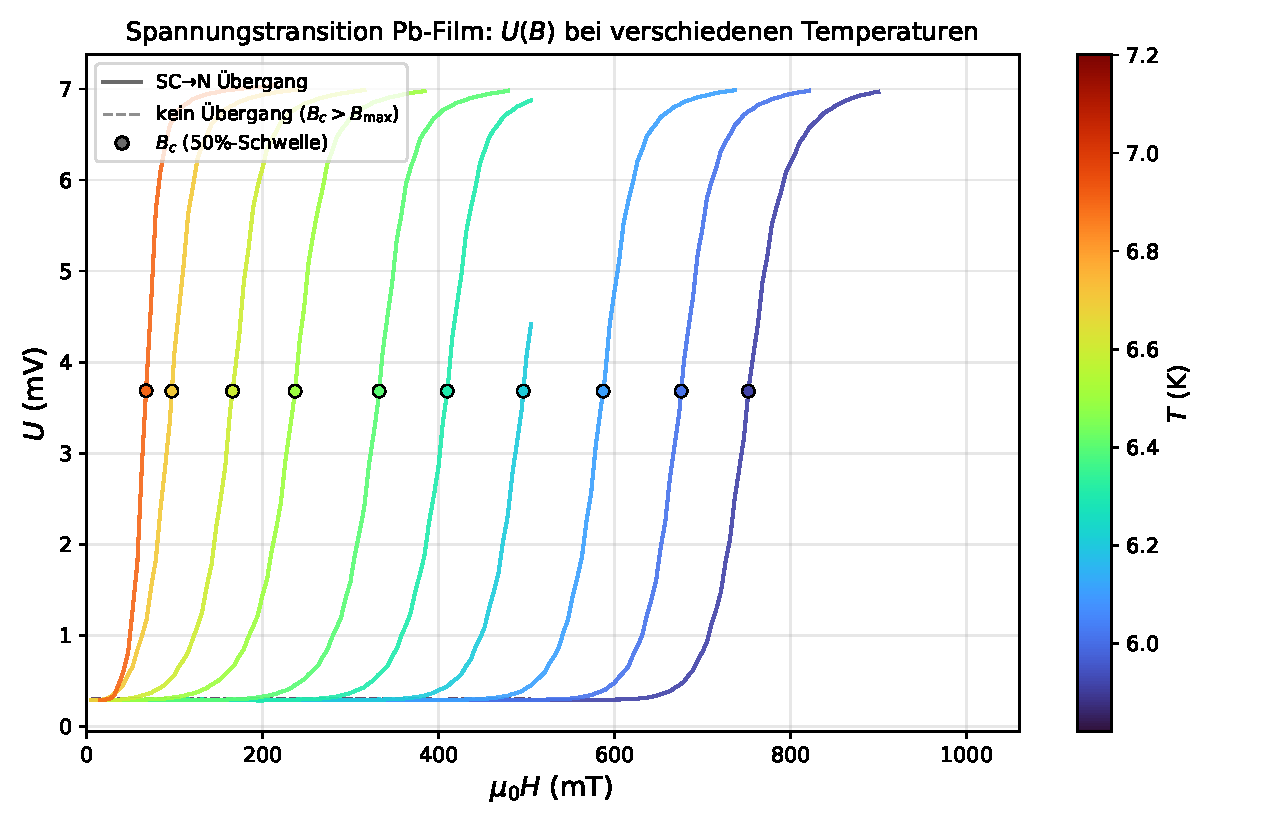
\includegraphics[width=0.9\linewidth]{../figures/fig_vb_curves.pdf}
    \caption{Spannungstransition $U(B)$ des Bleifilms bei verschiedenen Temperaturen
    (Farbkodierung: blau $= 5{,}82~\mathrm{K}$, rot $= 7{,}20~\mathrm{K}$).
    Durchgehende Linien: klarer SC-$\to$N-Übergang.
    Gepunktete Linien: kein Übergang im Messbereich oder Film bereits normal bei $B=0$.
    Kreissymbole markieren die extrahierten $B_c$-Werte (50\%-Schwelle).}
    \label{fig:vb_curves}
\end{figure}

\subsubsection*{Parabolisches Phasendiagramm}

Abbildung~\ref{fig:bc_phase} zeigt die so bestimmten $B_c(T)$-Werte zusammen mit dem Fit des parabolischen Gesetzes~\eqref{eq:bc_parabola}.
Insgesamt liegen 9 auswertbare Punkte im Temperaturbereich $5{,}916~\mathrm{K} \leq T \leq 6{,}901~\mathrm{K}$ vor; ein zusätzlicher Punkt bei $T = 5{,}821~\mathrm{K}$ liefert nur eine untere Schranke $B_c > 505~\mathrm{mT}$.

Die Anpassung von Gleichung~\eqref{eq:bc_parabola} an die 10 Messpunkte mit freien Parametern $B_c(0)$ und $T_c$ ergibt:
\begin{align}
    B_c(0) &= (2779 \pm 165)~\mathrm{mT}, \label{eq:fit_bc0} \\
    T_c     &= (6{,}861 \pm 0{,}038)~\mathrm{K}. \label{eq:fit_tc}
\end{align}
Die parabolische Form wird durch die Daten gut bestätigt (vgl.\ Abbildung~\ref{fig:bc_phase}).

\begin{figure}[htbp]
    \centering
    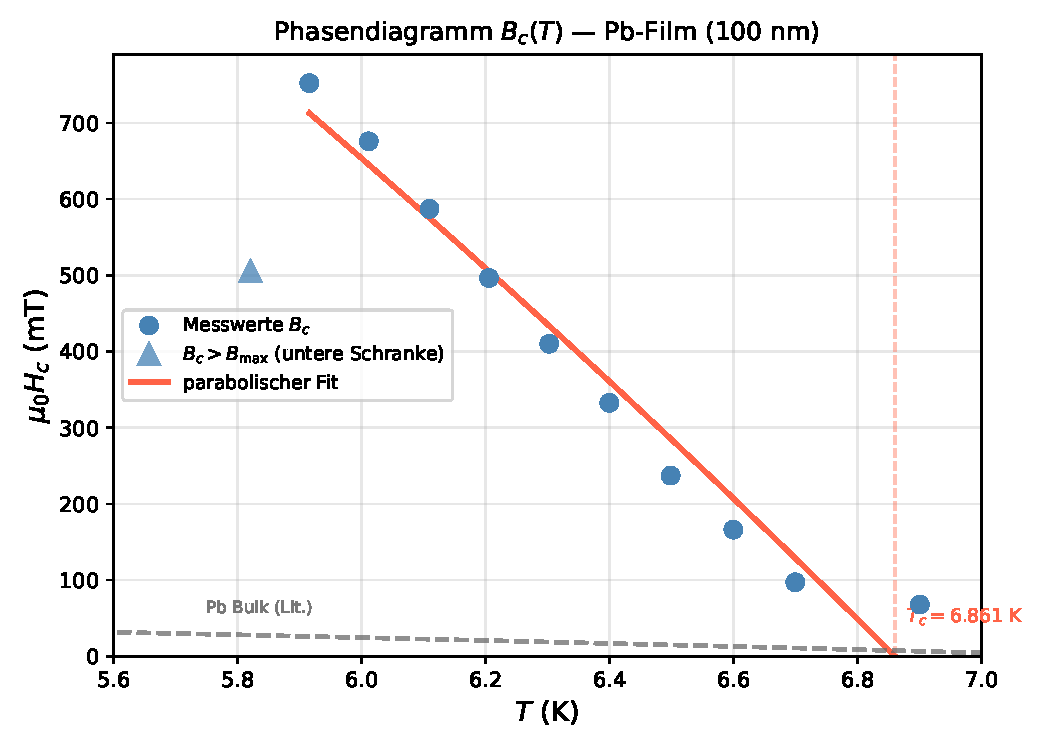
\includegraphics[width=0.88\linewidth]{../figures/fig_bc_phase.pdf}
    \caption{Magnetisches Phasendiagramm $B_c(T)$ des Pb-Films (100~nm).
    Kreise: auswertbare Messpunkte.
    Dreieck: untere Schranke bei $T = 5{,}82~\mathrm{K}$ ($B_c > 505~\mathrm{mT}$).
    Rote Kurve: parabolischer Fit~\eqref{eq:bc_parabola} mit $B_c(0) = 2779~\mathrm{mT}$, $T_c = 6{,}861~\mathrm{K}$.
    Gestrichelte schwarze Kurve: Pb-Bulk-Literaturwerte ($B_c(0) = 80~\mathrm{mT}$, $T_c = 7{,}2~\mathrm{K}$).}
    \label{fig:bc_phase}
\end{figure}

\subsection{Kritischer Strom $I_c(T)$}

\subsubsection*{I-V-Kennlinien}

Abbildung~\ref{fig:iv_curves} zeigt die gemessenen I-V-Kennlinien des Bleifilms bei acht Temperaturen zwischen $T = 6{,}499~\mathrm{K}$ und $T = 6{,}800~\mathrm{K}$.
Aufgetragen ist die Filmspannung abzüglich der SC-Basislinie ($U_0 \approx 290~\mu\mathrm{V}$) über dem Strom.
Bis zum kritischen Strom $I_c$ bleibt $\Delta U \approx 0$; darüber wächst $\Delta U$ steil an und geht in einen nahezu linearen Verlauf über, der dem Normalzustand entspricht.

\begin{figure}[htbp]
    \centering
    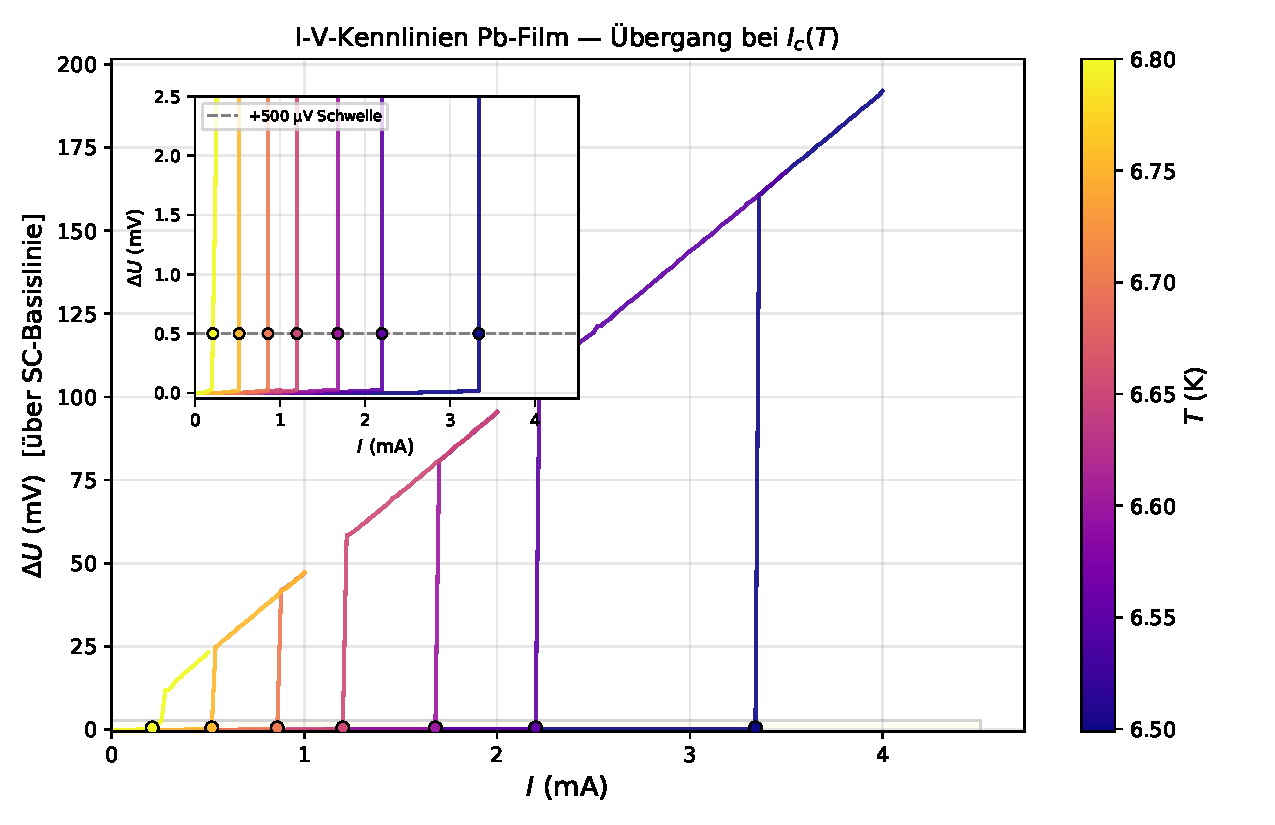
\includegraphics[width=0.9\linewidth]{../figures/fig_iv_curves.pdf}
    \caption{I-V-Kennlinien des Pb-Films bei verschiedenen Temperaturen
    (Farbkodierung: lila $= 6{,}499~\mathrm{K}$, gelb $= 6{,}800~\mathrm{K}$).
    Aufgetragen ist $\Delta U = U - U_0$ mit SC-Basislinie $U_0 \approx 290~\mu\mathrm{V}$.
    Kreissymbole: extrahierte $I_c$-Werte (Schwelle $\Delta U > 500~\mu\mathrm{V}$).}
    \label{fig:iv_curves}
\end{figure}

\subsubsection*{Temperaturabhängigkeit von $I_c$}

Abbildung~\ref{fig:ic_temp} zeigt die extrahierten $I_c(T)$-Werte.
Mit steigender Temperatur nimmt $I_c$ monoton ab.
Bei $T = 6{,}499~\mathrm{K}$ beträgt $I_c \approx 3{,}34~\mathrm{mA}$, bei $T = 6{,}800~\mathrm{K}$ nur noch $I_c \approx 212~\mu\mathrm{A}$.
Bei der Messung bei $T = 6{,}650~\mathrm{K}$ wurde der Strom nur bis $1~\mathrm{mA}$ erhöht, ohne dass ein Übergang eintrat; dieser Punkt liefert daher nur eine untere Schranke $I_c > 1~\mathrm{mA}$.

Unter Verwendung des aus dem $B_c(T)$-Fit bestimmten $T_c = 6{,}861~\mathrm{K}$ wird das Potenzgesetz
\begin{equation}
    I_c(T) = I_c(0)\left(1 - \frac{T}{T_c}\right)^n
    \label{eq:ic_fit}
\end{equation}
an die Daten angepasst (mit festgehaltenem $T_c$).
Dies liefert den Exponenten $n = 1{,}75 \pm 0{,}16$, konsistent mit dem theoretischen Ginzburg-Landau-Wert $n = 3/2$ für den Grenzfall nahe $T_c$.

\begin{figure}[htbp]
    \centering
    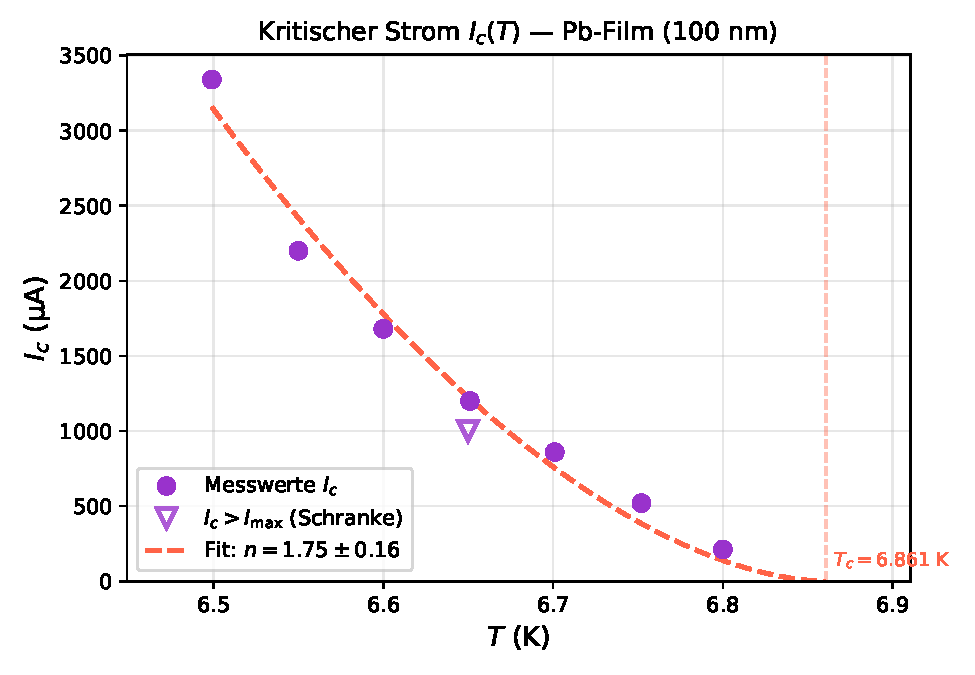
\includegraphics[width=0.82\linewidth]{../figures/fig_ic_temp.pdf}
    \caption{Kritischer Strom $I_c(T)$ des Pb-Films (100~nm).
    Kreise: Messwerte.
    Dreieck: untere Schranke bei $T = 6{,}650~\mathrm{K}$.
    Gestrichelte Kurve: Fit~\eqref{eq:ic_fit} mit festgehaltenem $T_c = 6{,}861~\mathrm{K}$ (aus $B_c(T)$-Fit) und $n = 1{,}75$.}
    \label{fig:ic_temp}
\end{figure}

\subsection{Levitation (qualitativ)}

Im Rahmen einer qualitativen Demonstration wurde ein Neodym-Permanentmagnet über eine gekühlte YBCO-Tablette gehalten und in mehreren Zentimetern Abstand zur Oberfläche frei schwebend beobachtet.
Das Experiment wurde sowohl im Zero-Field-Cooling- als auch im Field-Cooling-Modus durchgeführt.
Im Zero-Field-Cooling-Modus levitierte der Magnet stabil; im Field-Cooling-Modus war zwar die Levitation geringer, jedoch zeigte die Tablette deutliches Flux-Pinning: Der Magnet konnte innerhalb eines gewissen Bereichs lateral bewegt werden, ohne dass er herunterfiel.
Eine quantitative Auswertung (z.\,B.\ Levitationshöhe, Haltekraft) wurde nicht vorgenommen.

\newpage

% ============================================================
%  Kapitel 5 — Diskussion und Fazit
% ============================================================
\section{Diskussion und Fazit}
\label{sec:diskussion}

\subsection{Kritisches Feld $B_c(0)$ und Dünnfilmeffekt}

Der gemessene Wert $B_c(0) = (2779 \pm 165)~\mathrm{mT}$ liegt um mehr als eine Größenordnung über dem Bulk-Literaturwert für Blei ($B_c^\mathrm{Bulk}(0) = 80~\mathrm{mT}$~\cite{Buckel2013}).
Dies ist eine direkte Konsequenz der Dünnen-Film-Geometrie: Bei einem Film der Dicke $d = 100~\mathrm{nm}$ in senkrechtem Magnetfeld ist die relevante Eindringtiefe die Pearl-Länge~\cite{Pearl1964}
\begin{equation}
    \Lambda = \frac{2\lambda_L^2}{d} = \frac{2 \times (39~\mathrm{nm})^2}{100~\mathrm{nm}} \approx 30~\mathrm{nm}.
\end{equation}
Da $\Lambda \ll d$, ist der Film im Regime $d \gg \Lambda$; tatsächlich ist jedoch die entscheidende Längenskala die Kohärenzlänge $\xi_\mathrm{Pb}(0) \approx 83~\mathrm{nm}$~\cite{Tinkham2004}.
Für $d < \xi$ gelten besondere geometrische Bedingungen, die das effektive kritische Feld stark erhöhen können.
Der beobachtete Wert ist mit der Literatur zu dünnen Pb-Filmen qualitativ konsistent~\cite{Tinkham2004}.

\subsection{Sprungtemperatur $T_c$}

Der Fit liefert $T_c = (6{,}861 \pm 0{,}039)~\mathrm{K}$, also etwa $0{,}34~\mathrm{K}$ unterhalb des Bulk-Wertes $T_c^\mathrm{Bulk} = 7{,}2~\mathrm{K}$.
Eine Reduktion von $T_c$ in dünnen Filmen ist bekannt und kann durch Größeneffekte sowie Verunreinigungen beim Aufdampfen verursacht werden~\cite{Tinkham2004}.
Die direkte Beobachtung, dass Messungen bei $T \geq 6{,}796~\mathrm{K}$ und $B = 0$ keine Supraleitung mehr zeigen, ist konsistent mit dem Fit-Ergebnis.

\paragraph{Anomalie bei $T = 6{,}901~\mathrm{K}$.}
Auffällig ist, dass bei der unmittelbar davor liegenden Messung ($T = 6{,}900~\mathrm{K}$) der Film bereits vollständig normalleitend war, während bei $T = 6{,}901~\mathrm{K}$ ein Übergang bei $B_c \approx 68~\mathrm{mT}$ gemessen wurde.
Da beide Temperaturen innerhalb der Messgenauigkeit des Lakeshore~340 ($\pm 5~\mathrm{mK}$) identisch sind, ist davon auszugehen, dass die Temperatur während des Messzyklus leicht driftete.
Dieses Datenpunkt liegt im Fit nahe dem Rand des definierten Bereichs und beeinflusst die Ergebnisse nur geringfügig.

\subsection{Kritischer Strom und GL-Exponent}

Der Exponent $n = 1{,}75 \pm 0{,}16$ aus dem $I_c(T)$-Fit ist mit dem theoretischen Ginzburg-Landau-Wert $n = 3/2$ für den Grenzfall $T \to T_c$ verträglich.
Der Temperaturbereich der $I_c$-Messungen ($6{,}5~\mathrm{K}$ bis $6{,}8~\mathrm{K}$) liegt bereits sehr nah an $T_c = 6{,}861~\mathrm{K}$, sodass das Potenzgesetz~\eqref{eq:ic_fit} gut anwendbar ist.
Der absolute Wert $I_c(0)$ aus dem Fit ($\approx 548~\mathrm{A}$, extrapoliert auf $T = 0$) ist eine sehr starke Extrapolation über einen Temperaturbereich, in dem keine Daten vorliegen, und daher wenig aussagekräftig.

\subsection{Limitierungen und nicht durchgeführte Versuche}

Mehrere Versuchsteile konnten nicht abgeschlossen werden:
\begin{itemize}
    \item \emph{Pickup-Spule (Meißner-Effekt, Suszeptibilität)}: Der Versuchsaufbau war defekt.
    \item \emph{YBCO $R(T)$ in $ab$- und $c$-Richtung}: Kein Stickstoff-Kryostat verfügbar.
    \item \emph{Quantitative Levitation}: Nur qualitativ beobachtet, keine Messung.
\end{itemize}
Die fehlenden Teile schränken die Möglichkeit ein, Typ-I- und Typ-II-Supraleitung direkt am gleichen Versuchstag zu vergleichen.

\subsection{Fazit}

Trotz der eingeschränkten Versuchsdurchführung konnten die zentralen Eigenschaften der Typ-I-Supraleitung am Bleifilm quantitativ charakterisiert werden.
Das parabolische Gesetz $B_c(T) = B_c(0)[1-(T/T_c)^2]$ wurde über fast den gesamten Temperaturbereich unterhalb $T_c$ bestätigt.
Der erhöhte Wert von $B_c(0) \approx 2779~\mathrm{mT}$ gegenüber dem Bulk ist eine klare Manifestation des Dünnfilmeffekts im senkrechten Magnetfeld.
Die Sprungtemperatur $T_c = 6{,}861~\mathrm{K}$ liegt leicht unterhalb des Bulk-Wertes, was für aufgedampfte Pb-Filme typisch ist.
Die $I_c(T)$-Messungen bestätigen qualitativ den erwarteten Potenzgesetzverlauf mit einem GL-konsistenten Exponenten.
Das Levitationsexperiment demonstrierte anschaulich den Meißner-Effekt und das Flux-Pinning in YBCO.


% ---- Literatur ----
\newpage
\printbibliography[heading=bibintoc, title={Literatur}]

\end{document}
